% Chapter 1 of the pyformex manual

\chapter{Introduction}
\label{cha:introduction}

\section{What is \pyformex?}
\label{sec:what-pyformex}
You probably expect to find here a short definition of what \pyformex is and what it can do for you. I may have to disappoint you: describing the essence of \pyformex in a few lines is not an easy task to do, because the program can be (and is being) used for very different tasks. So I will give you two answers here: a short one and a long one.

The short answer is that \pyformex is a program to \emph{generate large structured sets of coordinates by means of subsequent mathematical transformations gathered in a script.}
If you find this definition too dull, incomprehensible or just not descriptive enough, read on through this section and look at some of the examples in this manual and on the \htmladdnormallinkfoot{\pyformex website}{\websiteURL}. You will then probably have a better idea of what \pyformex{} is. 

The initial intent of \pyformex was the rapid design of three-dimensional structures with a configuration that can easier be obtained through mathematical description than through interactive generation of its subparts and assemblage thereof. While during development of the program we have concentrated mostly on wireframe type structures, surface and solid elements have been part of \pyformex right from the beginning. Still, most of the examples included with \pyformex are of frame type and most of the practical use of the program is in this area.

The stent\footnote{A stent is a tube-shaped structure that is e.g. used to reopen (and keep open) obstructed blood vessels.} structure in the figure below is a good illustration of what \pyformex can do and what it was intended for. 

\begin{figure}[h]
  \centering
  \begin{makeimage}
  \end{makeimage}
  \begin{latexonly}
    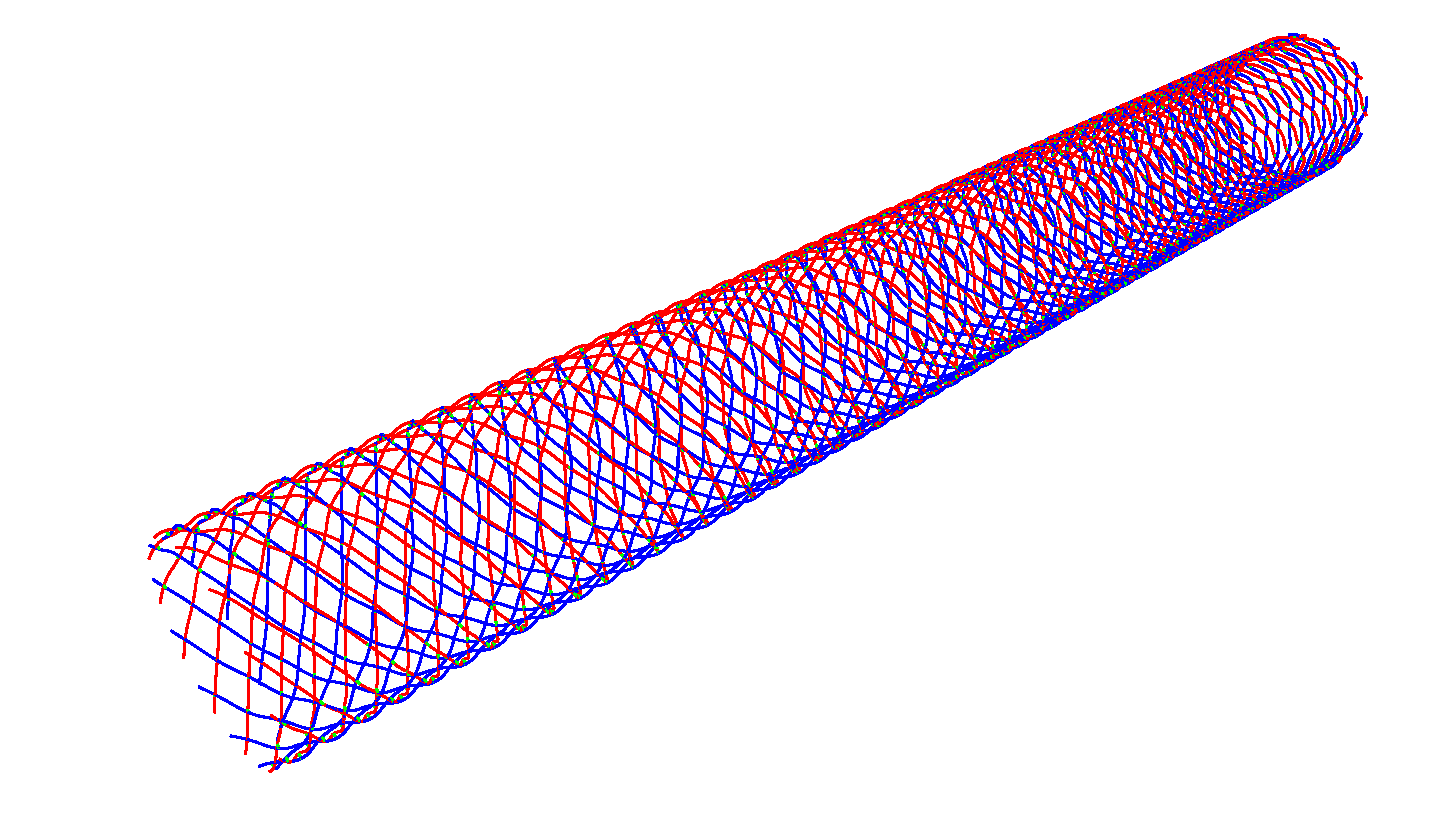
\includegraphics[width=12cm]{images/wirestent}
  \end{latexonly}
  \begin{htmlonly}
    \htmladdimg{../images/wirestent.png}
  \end{htmlonly}  
  \caption{WireStent example.}
\end{figure}

This structure is composed of 22032 line segments, each with 2 nodes. Nobody in his right mind would ever even try to input all the 132192 coordinates of all the points describing that structure. 
With \pyformex, one could define the structure by a sequence of operations like this:
 \begin{itemize}
 \item Create a planar base module of two crossing wires.
 \item Extend the base module with a mirrored and translated copy.
 \item Replicate the base module in both directions of the base plane.
 \item Roll the planar grid into a cylinder.
 \end{itemize}
 The procedure is illustrated by the subsequent images in the figure below.
 \begin{figure}[h]
   \centering
   \begin{makeimage}
   \end{makeimage}
   \begin{latexonly}
     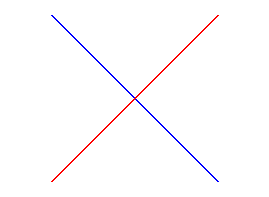
\includegraphics[width=2cm]{images/wirestent-1}
     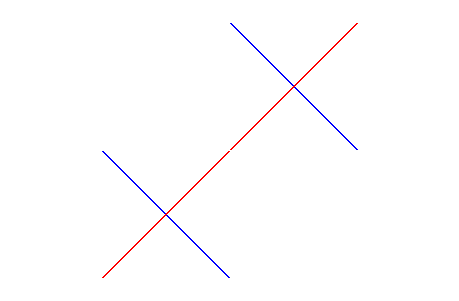
\includegraphics[width=2cm]{images/wirestent-2}
     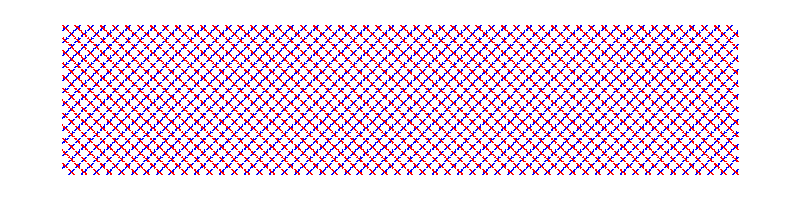
\includegraphics[width=12cm]{images/wirestent-3}
   \end{latexonly}
   \begin{htmlonly}
     \htmladdimg{../images/wirestent-1.png}
     \htmladdimg{../images/wirestent-2.png}
     \htmladdimg{../images/wirestent-3.png}
   \end{htmlonly}  
   \label{fig:WireStent steps}
   \caption{WireStent example.}
 \end{figure}


\section{Rationale}
\label{sec:rationale}

\section{History}
\label{sec:history}


\section{Installation}
\label{sec:installation}
\subsection{Installation on Linux platforms}
\label{sec:installation-linux}

%\subsection{Installation on Windows platforms}
%\label{sec:installation-windows}


\section{Quick tutorial for the \pyformex{} GUI}
\label{sec:gui-tutorial}
In the current version () the GUI mainly serves the following purposes:
\begin{itemize}
\item Display a structure in 3D. This includes changing the viewpoint, orientation and viewing distance. Thus you can interactively rotate, translate, zoom.
\item Save a view in one of the supported image formats. Most of the images in this manual and on the \pyformex{} website were created that way. 
\item Changing \pyformex settings (though there aren't many yet that can be changed through the GUI).
\item Running \pyformex scripts, possibly starting other programs and display their results.
\end{itemize}

The GUI does not (yet) provide a means to interactively design a structure, select parts of a structure or set/show information about (parts of) the structure. Designing a structure is done by writing a small script with the mathematical expressions needed to generate it. Any text editor will be suitable for this purpose. The author uses XEmacs, but this is just a personal preference. 
A Python aware editor is preferable though, because that is the language used in \pyformex scripts.
A \pyformex editor integrated into the GUI remains on our TODO list, but it certainly is not our top priority, because general purpose editors are adequate for most of our purposes. 

The best way to learn to use \pyformex is by studying and changing some of the examples. I suggest that you first take a look at the examples included in the \pyformex GUI and select those that display structures that look interesting to you. Then you can study the source code of those examples and see how the structures got built. 
When starting up, \pyformex reads through the Examples directory (this is normally the 'examples' subdirecty located under the pyformex installation dir).  
\menuselection{Examples \sub WireStent}


\section{Quick {Python tutorial}}
\label{sec:python-tutorial}
This could be part of the tutorial in chapter 2

\section{Quick NumPy tutorial}
\label{sec:numpy-tutorial}
This could be part of the tutorial in chapter 2

%%% Local Variables: 
%%% mode: latex
%%% TeX-master: "manual"
%%% End: 
